\subsection{Echo State Networks}

\begin{figure}[htp]
  \centering
  \subfloat[Training Flow]{
    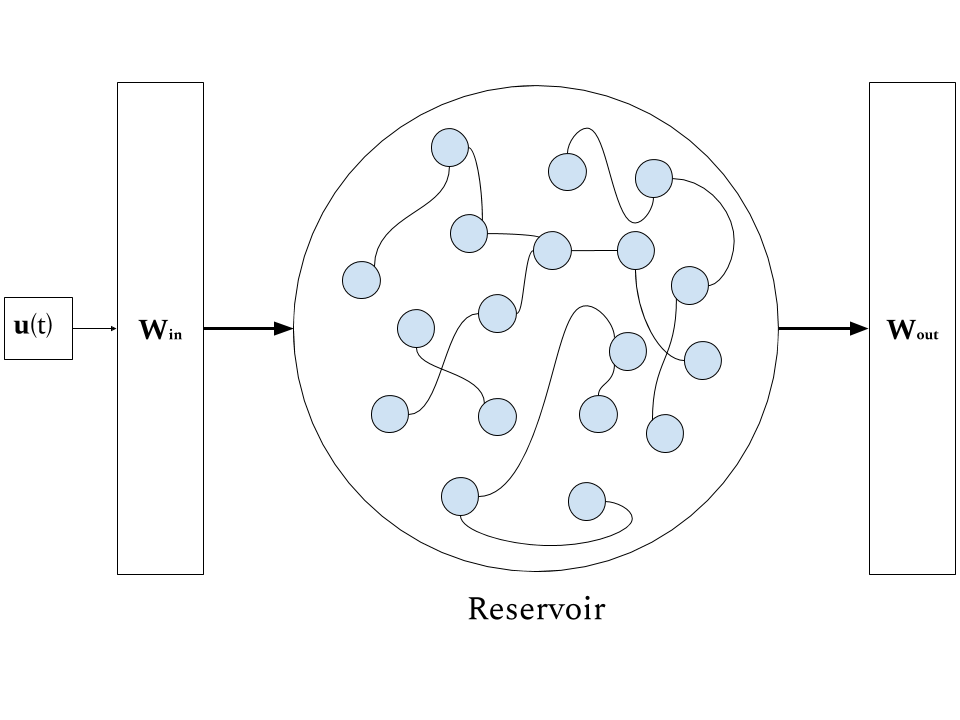
\includegraphics[clip, width=\columnwidth]{reservoir_training.png}
  }


  \subfloat[Predicting Flow]{
    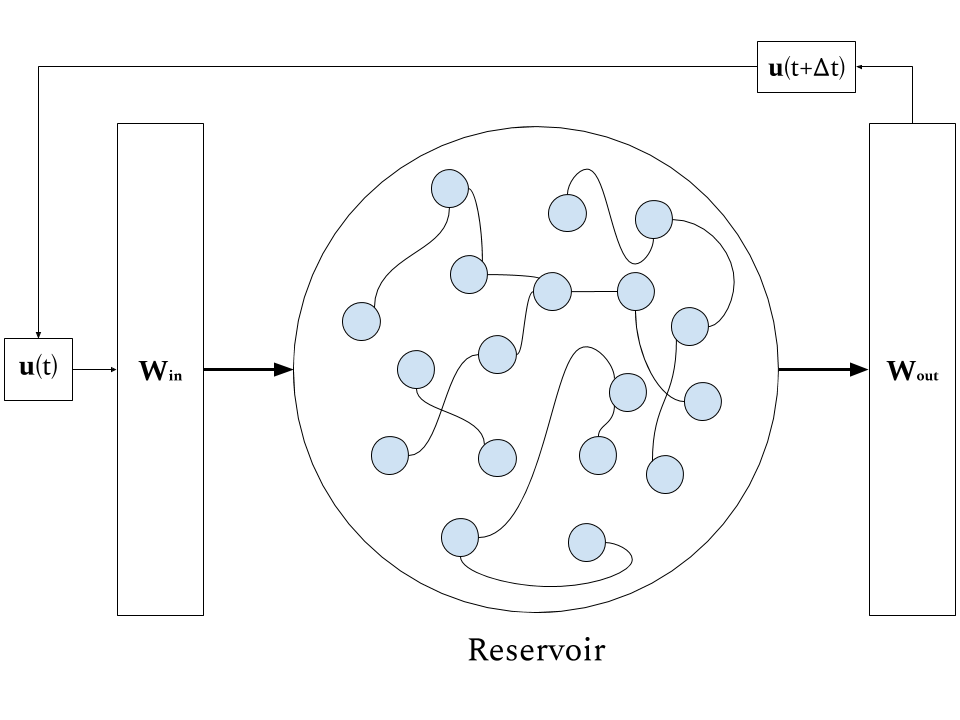
\includegraphics[clip, width=\columnwidth]{reservoir_predicting.png}
  }
  \caption{Reservoir behavior in the training and predicting phases.}
  \label{fig:reservoir_graph}
\end{figure}

An \gls{esn}, sometimes called ``reservoir computing,'' is a type of recurrent
neural network that replaces the many hidden layers of a conventional feed-
forward neural network with a reservoir that is
\begin{enumerate}
  \item sparse.
  \item connected by uniformly random weights, centered at zero.
  \item large (i.e. has many neurons).
\end{enumerate}

The reservoir is therefore a randomly instantiated adjacency matrix,
\textit{\textbf{W}}, of size $N \times N$. The input vector, $U(t)$, of
$K$ units is mapped onto the reservoir by an input matrix,
 $W^{in}$ of size $N \times K$. The activation states of the reservoir are calculated by
 \begin{align}
   x(t) &= \tanh \left(W^{in}\cdot U(t) + \mathbf{W}x(t-1)\right)
 \end{align}
 Where $x(t)$ is the collection of reservoir activations.
 The output is read by an output weight matrix,
 $W^{out}$.
 \begin{align}
   y(t) &= \left(W^{out}\right)^T\cdot x(t)
 \end{align}
 This output matrix functions like a single layer feed-forward
 neural network. In the training phase, the output, $U(t+\Delta t)$, is
 discarded and the next training input passed to the network. During the
 prediction phase, the output is kept and used as the next input. This behavior
 is shown in Figure \ref{fig:reservoir_graph}. The speed of \glspl{esn} is owed
 to this structure; only $W^{out}$ has tunable weights. Everything else is
 fixed.
